\documentclass{article}
\usepackage{geometry}
\geometry{hmargin=2.5cm}
\usepackage{fancyhdr}
\usepackage{amsmath}
\usepackage{graphicx}
\usepackage{subcaption}
\usepackage{float}
\usepackage{hyperref}
\usepackage{gensymb}
\usepackage{siunitx}


\title{Capteurs}
\date{2019 -- 2020}
\author{Laura Binacchi}

\begin{document}
\pagenumbering{gobble}
\maketitle
\newpage
\tableofcontents
\pagenumbering{arabic}
\newpage
    \section{Définition}
        \paragraph{}
        Un capteur est un élément qui transforme l'état d'une grandeur physique (mesurande) en une grandeur exploitable. C'est le premier élément d'une chaîne de mesurage.

        \paragraph{}
        Il existe deux types de capteurs : actifs et passifs.

    \section{La mesure}
        \paragraph{La mesure} est l'attribution d'une valeur numérique à une grandeur physique.

        \paragraph{Une grandeur physique} est la propriété d'un phénomène ou d'un corps que l'on peut quantifier.

        \paragraph{Mesurer une grandeur} c'est la comparer à une autre de grandeur de même espèce choisie comme unité de mesue.

        \paragraph{Une unité de mesure} est une grandeur particulière choisie comme grandeur de référence.

        \subsection{Les grandeurs physiques de base}
            \paragraph{}
            Par le système international d'unités (SI). On distingue les unités de base et les unités dérivées.
            \begin{table}[H]
            \begin{center}
                \caption{Les grandeurs physiques de base du SI.}
                \begin{tabular}{l|c|c|c}
                    \textbf{} & \textbf{Unité} & \textbf{Symbole} & \textbf{Symbole de}\\
                    \textbf{} & \textbf{de base} & \textbf{de l'unité} & \textbf{la dimension}\\
                    \hline
                    \textbf{Longueur} & mètre & \si{\meter} & L\\
                    \textbf{Masse} & kilogramme & \si{\kilogram} & M\\
                    \textbf{Temps} & seconde & \si{\second} & T\\
                    \textbf{Intensité électrique} & ampère & \si{\ampere} & I\\
                    \textbf{Température} & kelvin & \si{\kelvin} & $\Theta$\\
                    \textbf{Quantité de matière} & mole & \si{\mol} & N\\
                    \textbf{Intensité lumineuse} & candela & \si{\candela} & J\\
                \end{tabular}
            \end{center}
            \end{table}

        \subsection{Définition des étalons}
            \paragraph{}
            Depuis le 20 mai 2019, le système d'unités est établi à partir de constantes universelles afin de rendre le système d'unités le plus invariable et le plus universel possible.

                \subsubsection{Constantes de base}
                Notre SI compte sept unités de bases définies par sept constantes :
                \begin{itemize}
                    \item La fréquence de transition entre deux niveaux de l'état fondamental de l'atome de césium 133 (notée Cs).
                    \item La vitesse de la lumière dans le vide (notée c).
                    \item La constante de Planck (notée h) introduite par la mécanique quantique.
                    \item La charge élémentaire (notée e) de l'électromagnétisme.
                    \item La constante de Boltzmann (notée k) introduite en thermodynamique.
                    \item La constante d'Avogadro (notée NA) particulièrement utilisée en chimie.
                    \item Le rendement lumineux (noté Kcd) utilisé en photométrie.
                \end{itemize}

                \begin{figure}[H]
                    \centering
                    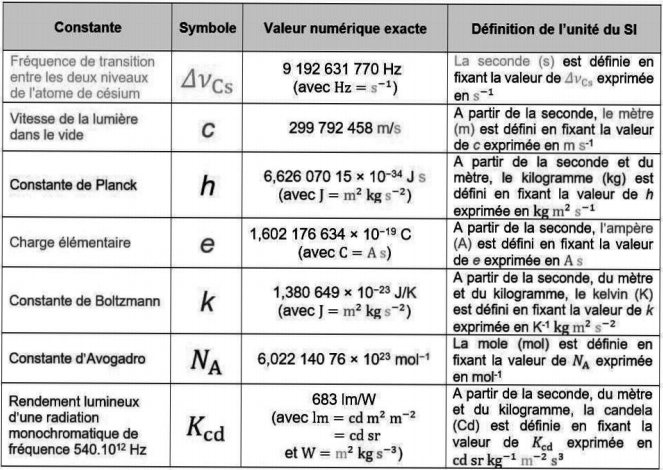
\includegraphics[width=0.7\linewidth]{./images/009-constantes-SI.png}
                    \caption{Les constantes de base du SI.}
                \end{figure}

                \subsubsection{Grandeur dérivées}
                \begin{table}[H]
                    \begin{center}
                        \caption{Les grandeurs physiques dérivées du SI.}
                        \begin{tabular}{l|c|c|c}
                            \textbf{}           & \textbf{}     & \textbf{Unité}    & \textbf{}         \\
                            \textbf{Grandeur}   & \textbf{Nom}  & \textbf{Symbole}  & \textbf{Expression}\\
                            \hline
                            fréquence           & hertz         & \si{\hertz}   & \SI{1}{\per\second}\\
                            \hline
                            force               & newton        & \si{\newton}  & \SI{1}{\kilogram \metre \per \square \second}\\
                            \hline
                            pression            & pascal        & \si{\pascal}  & \SI{1}{\newton \per \square \meter}\\
                            \hline
                            énergie, travail, quantité de chaleur & joule & \si{\joule} & \SI{1}{\newton \meter}\\
                            \hline
                            puissance, flux énergétique & watt & \si{\watt} & \SI{1}{\joule \per \second}\\
                            \hline
                            charge électrique, & coulomb & \si{\coulomb} & \SI{1}{\ampere \second}\\
                            quantité d'électricité &  &  & \\
                            \hline
                            potentiel électrique, différence de potentiel,& volt & \si{\volt} & \SI{1}{\watt \per \ampere}\\
                            tension, force électromotrice &  &  & \\
                            \hline
                            capacité électrique & farad & \si{\farad} & \SI{1}{\coulomb \per \volt}\\
                            \hline
                            résistance électrique & ohm & \si{\ohm} & \SI{1}{\volt \per \ampere}\\
                            \hline
                            conducante électrique & siemens & \si{\siemens} & \SI{1}{\per \ohm}\\
                            \hline
                            flux d'induction magnétique & weber & \si{\weber} & \SI{1}{\volt \second}\\
                            \hline
                            induction magnétique & tesla & \si{\tesla} & \SI{1}{\weber \per \square \meter}\\
                            \hline
                            inductance & henry & \si{\henry} & \SI{1}{\weber \per \ampere}\\
                            \hline
                            température Celsius & degré Celsius & \si{\celsius} & \SI{1}{\kelvin}\\
                            \hline
                            flux lumineux & lumen & \si{\lumen} & \SI{1}{\candela \per \steradian}\\
                            \hline
                            éclairement & lux & \si{\lux} & \SI{1}{\lumen \per \square \meter}\\
                        \end{tabular}
                    \end{center}
                    \end{table}

                
    \section{Dimension d'une grandeur dérivée}
    \paragraph{}
    La dimension exprime la relation existant entre une grandeur dérivée et les grandeurs de base dont elle dépend.
    \begin{equation*}
        dim G = \left[G\right] = L^\alpha M^\beta T^\gamma I^\delta \Theta^\epsilon N^\mu J^\nu
    \end{equation*}
    NB
    \begin{itemize}
        \item Si $G = 1$, la grandeur est dite sans dimension mais elle peut avoir une unité (e.g. les angles, rapport de deux grandeurs).
        \item Les dimensions des grandeurs sont indépendantes du système d'unité choisi.
        \item La dimension peut être utilisée pour vérifier des formules ou prédire le résultat d'une opération.
    \end{itemize}

        \subsection{Équations aux dimensions}
        \paragraph{}
        Les équations doivent toujours être homogènes, i.e.  que chaque membre d'une équation doit avoir la même dimension physique.

            \subparagraph{Exemples}
            \begin{itemize}
                \item L'équation aux dimensions de la force est
                \begin{equation*}
                    F = MLT^{-2}
                \end{equation*}
                puisque $F = m.a$ et l'unité SI est le $\si{\kilogram \meter \per \square \second}$ ou Newton.
                \item Pour l'énergie, l'équation aux dimensions est
                \begin{equation*}
                    F = ML^2T^{-2}
                \end{equation*}
                puisque $ W = \frac{1}{2}m.v^2$ et l'unité SI est le $\si{\kilogram \square \meter \per \square \second}$ ou Joule.
            \end{itemize}

        \subsection{Système SI}
        \begin{table}[H]
        \centering
        \begin{tabular}{c|c|c}
            & & \textbf{Puissance de 10}\\
            \textbf{Préfixe} & \textbf{Symbole} & \textbf{de l'unité}\\
            \hline
            exa & \si{\exa} & $10^{18}$\\
            \hline
            peta & \si{\peta} & $10^{15}$\\
            \hline
            tera & \si{\tera} & $10^{12}$\\
            \hline
            giga & \si{\giga} & $10^{9}$\\
            \hline
            mega & \si{\mega} & $10^{6}$\\
            \hline
            kilo & \si{\kilo} & $10^{3}$\\
            \hline
            hecto & \si{\hecto} & $10^{2}$\\
            \hline
            deca & \si{\deca} & $10^{1}$\\
            \hline
            & & $10^{0} = 1$\\
            \hline
            deci & \si{\deci} & $10^{-1}$\\
            \hline
            centi & \si{\centi} & $10^{-2}$\\
            \hline
            milli & \si{\milli} & $10^{-3}$\\
            \hline
            micro & \si{\micro} & $10^{-6}$\\
            \hline
            nano & \si{\nano} & $10^{-9}$\\
            \hline
            pico & \si{\pico} & $10^{-12}$\\
            \hline
            femto & \si{\femto} & $10^{-15}$\\
            \hline
            atto & \si{\atto} & $10^{-18}$\\
        \end{tabular}
        \end{table}

        \subsection{Radian et stéradian}
            \paragraph{}
            La radian est l'unité qui mesure les angles plan. Le stéradian est l'unité qui mesure les angles solides.

            \begin{figure}[H]
                \centering
                \begin{subfigure}[b]{0.15\linewidth}
                    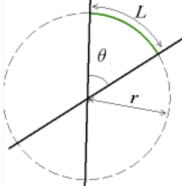
\includegraphics[width=\linewidth]{./images/010-radian.png}
                    \caption{$\theta = \frac{L}{R}$}
                \end{subfigure}
                \begin{subfigure}[b]{0.15\linewidth}
                    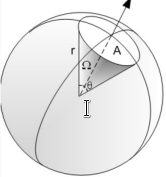
\includegraphics[width=\linewidth]{./images/011-steradian.png}
                    \caption{$\Omega = \frac{A}{R^2}$}
                \end{subfigure}
            \end{figure}
            \begin{table}[H]
            \centering
            \begin{tabular}{l|l}
                $\theta$ : angle exprimé en radian [\si{\radian}] & $\Omega$ : angle solide en stéradian [\si{\steradian}]\\
                L : longueur de la section du cercle [\si{\meter}] & A : surface de la section de sphère [\si{\square \meter}]\\
                R : rayon du cercle [\si{\meter}] & R : rayon de la sphère au carré [\si{\meter}]\\
            \end{tabular}
            \end{table}

        \subsection{Le Kelvin}
            \paragraph{}
            L'échelle des températures Celsius est, par définition, la température absolue décalée en origine de \SI{273,15}{\kelvin}.
            $$T_K = T_C + 273,15$$
            
            \paragraph{}
            On en déduit que :
            \begin{itemize}
                \item Le zéro absolu est situé à \SI{-273,15}{\celsius}.
                \item Les températures en kelvin ne sont jamais négatives.
                \item Les intervalles de l'échelle du degré Celsius sont identiques à ceux du Kelvin.
            \end{itemize}

        \subsection{La pression}
            \paragraph{}
            $$P = \frac{F}{S}$$
            \begin{itemize}
                \item P : pression en Pascal [\si{\pascal}]
                \item F : force en Newton [\si{\newton}]
                \item S : surface [\si{\square \meter}]
            \end{itemize}

            \paragraph{}
            On a $\SI{1}{\bar} = 10^5 \si{\pascal}$ et 1 atm $= \SI{1,013}{\bar}$. L'eau de ville est entre 2 et 5 bar, les pneus de voiture entre 1,5 et 2,5 bar, etc.

            \begin{figure}[H]
                \centering
                \begin{subfigure}[b]{0.3\linewidth}
                    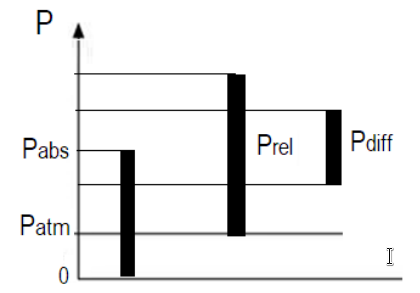
\includegraphics[width=\linewidth]{./images/012-pressions.png}
                \end{subfigure}
                \begin{subfigure}[b]{0.25\linewidth}
                    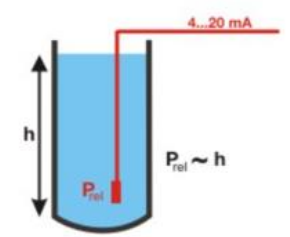
\includegraphics[width=\linewidth]{./images/013-pressions.png}
                \end{subfigure}
            \end{figure}

            \paragraph{La pression absolue} (Pabs) est la pression mesurée en référence à une pression nulle (vide absolu).

            \paragraph{La pression manométrique ou relative} (Pressure Gauge) donne la différence entre la pression d'un fluide et la pression atmosphérique (Patm).
            $$P_{abs} = P_{gauge} + P_{atm}$$

            \subsection{Pression hydrostatique}
            \paragraph{}
            L'hydrostatique est l'étude des fluides immobiles.

            \paragraph{Théorème}
            Dans un liquide en équilibre de masse volumique uniforme, la différence de pression entre deux points 1 et 2, situés respectivement à une profondeur h1 et h2 est donnée par : $$P_2 - P_1 = \rho.g.\Delta h$$

            \begin{itemize}
                \item $P$ : pression [\si{\pascal}]
                \item $\rho$ : masse volumique du liquide [\si{\kilogram \per \meter^{3}}]
                \item $g$ : accélération de la pesanteur [\si{\meter \per \second^{2}}]
            \end{itemize}
            
            \begin{figure}[H]
            \centering
                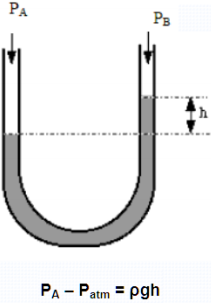
\includegraphics[width=0.2\linewidth]{./images/014-hydrostatique.png}
            \end{figure}

        \subsection{Débit volumique}
            \paragraph{}
            C'est la grandeur physique qui caractérise le volume d'un fluide qui traverse une surface donnée par unité de temps. C'est aussi le produit de la vitesse du fluide $u$ par sa section $S$ de passage (écoulement uniforme).
            $$Q_v = \frac{V}{t} = u.S$$

            \begin{itemize}
                \item $Q$ : débit en mètre cube par seconde [\si{\meter^3 \per \second}]
            \end{itemize}

            \paragraph{NB} La masse volumique est l'inverse du volume massique.

        \subsection{Masse volumique d'une substance}
            \paragraph{}
            C'est une grandeur physique qui caractérise la masse d'une substance par unité de volume.
            $$\rho = \frac{m}{V}$$
            \begin{itemize}
                \item $\rho$ : masse volumique [\si{\meter^3 \per \kilogram}]
                \item $m$ : masse de la substance homogène [\si{\kilogram}]
                \item $V$ : volume occupé [\si{\meter^3}]
            \end{itemize}

        \subsection{Diagramme de phase}
            \paragraph{}
            Ce diagramme permet de représenter les changements d'état d'un système en fonction de variables : température, pression, volume.

            \paragraph{Exemple de l'eau}
            \
            \begin{figure}[H]
            \centering
                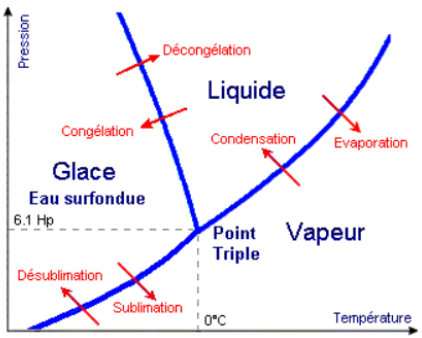
\includegraphics[width=0.45\linewidth]{./images/015-diagramme-phase-eau.png}
            \end{figure}

            \paragraph{NB}
            Point triple de l'eau (\SI{611}{\pascal} ; \SI{0}{\celsius}) ou (\SI{6,11}{\milli\bar} ; \SI{273,2}{\kelvin})

        \subsection{Les ondes}
            \paragraph{}
            Une onde est une vibration qui se propage sans transport de matière. Les vitesses de propagation (on parle de célérité de l'onde) d'une onde dépendent du milieu matériel de propagation et du type de l'onde. Une onde peut être absorbée, réfractée et/ou réfléchie.

            \paragraph{}
            La distance $d$ parcourue par une onde est $d = c.t$. La longueur d'onde $\lambda$ est la distance parcourue pendant un période $T$
            $$\lambda = c.T = \frac{c}{f}$$
            c = vitesse de la lumière = $3.10^8\si{\meter\per\second}$

            \paragraph{}
            On distingue
                \subparagraph{Les ondes mécaniques} qui se propagent à travers une matière physique dont la substance se déforme. E.g. ondes sonores.
                \subparagraph{Les ondes électromagnétiques} qui ne nécessitent pas de support physique : oscillations périodiques de champs électriques et magnétiques générés à l'origine par des particules chargées.

            \subsubsection{Classification des ondes électromagnétiques}
            \begin{table}[H]
                \centering
            \begin{tabular}{c|c|c}
                \textbf{Longueur d'onde} & & \\
                \textbf{(dans le vide)} & \textbf{Domaine} & \textbf{Fréquence}\\
                \hline
                $\lambda > \SI{30}{\centi\metre}$ & radio & $f < \SI{1}{\giga\hertz}$\\
                \hline
                $\SI{30}{\centi\meter} > \lambda > \SI{3}{\milli\meter}$ & micro-ondes (Wi-Fi, & $\SI{1}{\giga\hertz} < f < \SI{100}{\giga\hertz}$\\
                & téléphone portable, & \\
                & radar, etc). & \\
                \hline
                $\SI{3}{\milli\meter} > \lambda > \SI{700}{\nano\meter}$ & infrarouge & $\SI{100}{\giga\hertz} < f < \SI{430}{\tera\hertz}$\\
                \hline
                $\SI{700}{\nano\meter} > \lambda > \SI{400}{\nano\meter}$ & lumière visible & $\SI{430}{\tera\hertz} < f < \SI{750}{\tera\hertz}$\\
                \hline
                $\SI{400}{\nano\meter} > \lambda > \SI{10}{\nano\meter}$ & ultraviolet & $\SI{750}{\tera\hertz} < f < \SI{30}{\peta\hertz}$\\
                \hline
                $\SI{10}{\nano\meter} > \lambda > \SI{10}{\pico\meter}$ & rayon X & $\SI{30}{\peta\hertz} < f < \SI{30}{\exa\hertz}$\\
                \hline
                $\SI{10}{\pico\meter} > \lambda$ & rayon $\gamma$ & $\SI{30}{\exa\hertz} < f$\\
            \end{tabular}
            \end{table}

            \subsubsection{Optoélectronique}
            \begin{figure}[H]
            \centering
                \begin{subfigure}[]{0.5\linewidth}
                    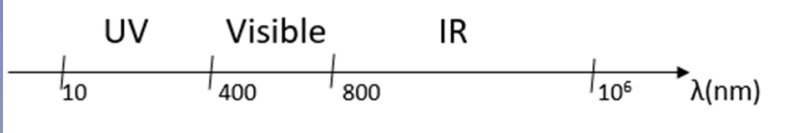
\includegraphics[width=\linewidth]{./images/016-optoelectronique.png}
                \end{subfigure}
                \begin{subfigure}[]{0.5\linewidth}
                    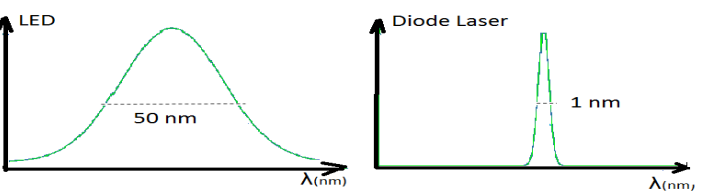
\includegraphics[width=\linewidth]{./images/017-optoelectronique.png}
                \end{subfigure}
            \end{figure}

            \subsubsection{La lumière}
            \begin{figure}[H]
            \centering
                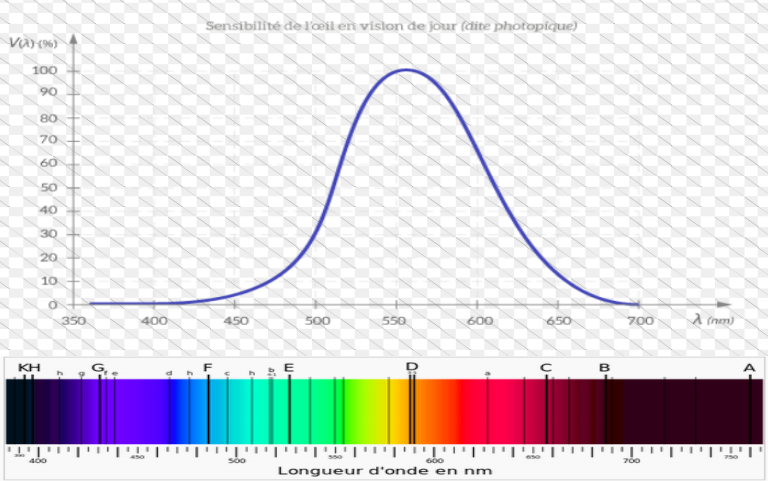
\includegraphics[width=0.6\linewidth]{./images/018-lumiere.png}
            \end{figure}
            La lumière est l'ensemble des ondes électromagnétiques visibles par
            l'œil humain.

            \subsubsection{Le lumen}
                \paragraph{}
                Le lumen (\si{\lumen}) est l'unité de flux lumineux. Il indique la quantité totale de lumière émise par seconde. C'est une unité de puissance comme le Watt.
                \begin{table}[H]
                \centering
                \begin{tabular}{l|c|c|c}
                    \textbf{Type de lampe} & \textbf{200-300}\si{\lumen} & \textbf{300-500\si{\lumen}} & \textbf{500-700\si{\lumen}}\\
                    \hline
                    \textbf{Ampoules à incandescence} & 25-30\si{\watt} & 40\si{\watt} & 60\si{\watt}\\
                    \hline
                    \textbf{Ampoules halogènes} & 18-25\si{\watt} & 35\si{\watt} & 50\si{\watt}\\
                    \hline
                    \textbf{Ampoules CLF} & 5-6\si{\watt} & 8\si{\watt} & 11\si{\watt}\\
                    \hline
                    \textbf{Ampoules LED} & 2-4\si{\watt} & 3-5\si{\watt} & 5-7\si{\watt}\\
                    \hline
                \end{tabular}
                \end{table}

                \begin{figure}[H]
                    \centering
                    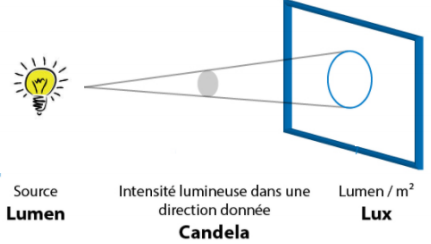
\includegraphics[width=0.5\linewidth]{./images/019-lumen.png}
                \end{figure}

                \paragraph{Le lumen} (\si{\lumen}) est l'unité de flux lumineux. Il indique la quantité totale de lumière émise par seconde.
                \paragraph{Le candela} (\si{\candela}) est l'unité d'intensité lumineuse : \SI{1}{\candela} = \SI{1}{\lumen \per \steradian}. Un candela correspond à la luminosité d'une bougie.
                \paragraph{Le lux} (\si{\lux}) est l'unité d'éclairement : \SI{1}{\lux} = \SI{1}{\lumen \per \square \meter}.

            \subsubsection{Les ondes sonores}
                \paragraph{}
                L'onde sonore est une variation de la pression de l'air. La propagation des ondes sonores nécessite un support matériel. C'est une onde mécanique.


                \begin{figure}[H]
                    \centering
                    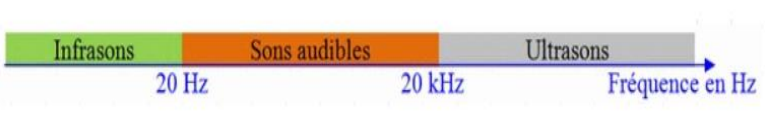
\includegraphics[width=0.6\linewidth]{./images/020-ondes-sonores.png}
                \end{figure}

                \paragraph{}
                Vitesse de propagation d'une onde sonore :
                \begin{itemize}
                    \item $v \approx \SI{340}{\meter \per \second}$ dans l'air;
                    \item $v = \SI{1500}{\meter \per \second}$ dans l'eau;
                    \item $v = \SI{5000}{\meter \per \second}$ dans l'acier.
                \end{itemize}


    \newpage
    \section{Caractéristiques d'un capteur}

        \subsection{Fidélité}
            \paragraph{}
            La fidélité désigne l'étroitesse de l'accord entre les mesures répétées du même objet dans certaines conditions (voire répétabilité et reproductibilité). On a une bonne fidélité de mesure si la dispersion est faible.

            \paragraph{}
            Écart-type ou variance.

            \paragraph{Répétabilité}
            Mesures effectuées dans des conditions identique : même laboratoire, même opérateur, même système de mesure, intervalle très court.

            \paragraph{Reproductibilité}
            Les conditions de mesure sont différentes : moments différents, etc.

        \subsection{Justesse}
            \paragraph{}
            La justesse est l'étroitesse de l'accord entre la moyenne des mesures et une valeur de référence. La justesse est bonne quand l'erreur systématique est faible.

            \paragraph{Biais}
            Le biais de mesure ou erreur de justesse est l'estimation de l'erreur systématique :
            \begin{equation*}
                Biais = <Y> - Y_{ref}
            \end{equation*}

            \subsubsection{Fidélité vs justesse}
            \begin{figure}[H]
                \centering
                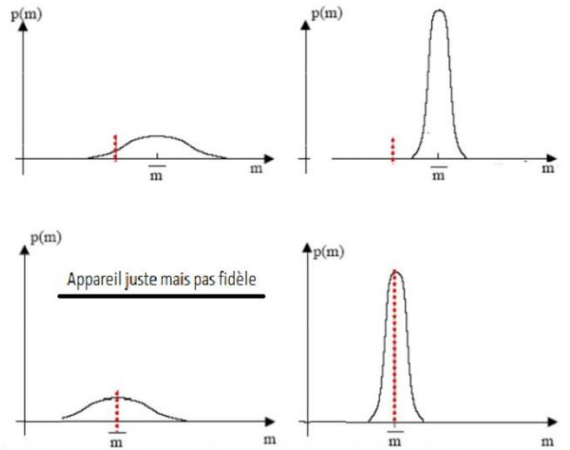
\includegraphics[width=0.6\linewidth]{./images/001-fidelite-vs-justesse.png}
                \caption{Fidélité vs justesse}
                \label{fig:fidelite-vs-justesse}
            \end{figure}

        \subsection{Précision}
            \paragraph{}
            La précision est définie par l'écart en pourcentage que l'on peut obtenir entre la valeur réelle et la valeur obtenue en sortie du capteur. La précision est souvent donnée en pourcentage de l'étendue de mesure. Un capteur précis est juste et fidèle.

            \paragraph{Exemple}
            L'erreur maximum commise par ce capteur est de $\pm 0.5\degree C$ (cf dossier).
            \begin{figure}[H]
                \centering
                \begin{subfigure}[b]{0.35\linewidth}
                    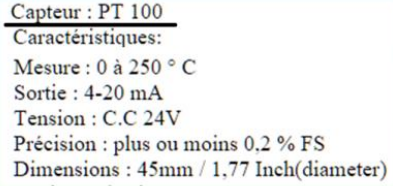
\includegraphics[width=\linewidth]{./images/002-precision-pt-100.png}
                \end{subfigure}
                \begin{subfigure}[b]{0.2\linewidth}
                    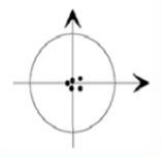
\includegraphics[width=\linewidth]{./images/003-precision-pt-100.png}
                \end{subfigure}
            \end{figure}
            
        \subsection{Sensibilité}
        \paragraph{} La sensibilité est le coefficient qui lie la grandeur physique d'entrée à mesurer à la grandeur électrique de sortie. Plus un capteur est sensible, plus la mesure pourra être précise.

        \paragraph{Exemple}
        Pour un capteur de pression :
        \begin{equation*}
            V_{\left(p\right)} = a . p + V_0\\
            \Rightarrow S_c = \frac{dV}{dp} = a
        \end{equation*}
        Prenons une sensibilité $a = \SI{10}{\milli\volt/\hecto\pascal}$ $\Rightarrow V_{\left(p\right)} = 10p + V_0$.

        \subsection{Linéarité}
        \paragraph{}
        Un capteur est linéaire si sa sensibilité est constante.

        \paragraph{Exercice}
        Ces capteur sont-ils linéaires ?
        \begin{itemize}
            \item PT 100 : $R_{\left(T\right)} = R0\left(1 + aT\right)$
            \item Thermistance : $R_{\left(T\right)} = a.e^{\frac{b}{T}}$
        \end{itemize}

            \subsubsection{Erreur de linéarité}
            \begin{figure}[H]
                \centering
                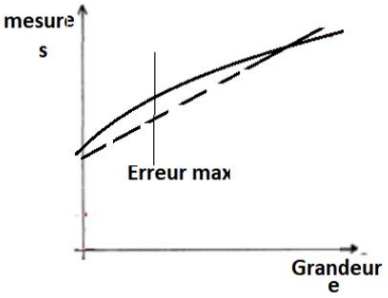
\includegraphics[width=0.35\linewidth]{./images/004-erreur-linearite.png}
                \caption{Erreur de linéarité}
            \end{figure}

            \paragraph{}
            L'erreur de linéarité est la valeur absolue de l'écart maximum entre la courbe caractéristique du capteur (par valeurs montantes) et la droite de référence. Pour déterminer l'erreur de linéarité, une série de mesures est prise par valeurs montantes jusqu'à la valeur nominale.

            \subsubsection{Erreur de réversibilité}
            \begin{figure}[H]
                \centering
                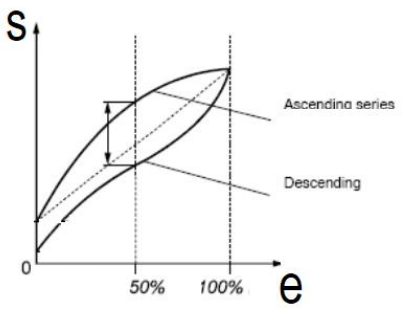
\includegraphics[width=0.4\linewidth]{./images/005-erreur-reversibilite.png}
                \caption{Erreur de réversibilité}
            \end{figure}

            \paragraph{}
            C'est une mesure d'hystérésis : une mesure de la différence entre les courbes caractéristiques déterminées au couple croissant et décroissant.

        \subsection{Résolution}
        \paragraph{}
        La résolution est la plus petite variation de grandeur mesurable par le capteur. Plus elle est faible, meilleure est cette résolution.

        \paragraph{Exemple}
        Pour un pH-mètre dont l'intervalle de mesure est de 0 à 14 (acide à base), la résolution est de 0.01 : le nombre récolté varie par pas de 0.01.

        \subsection{Plage de mesure}
        \paragraph{}
        La plage de mesure d'un capteur est l'étendue des valeurs d'entrée qu'il peut traiter sans dégrader son fonctionnement.

        \paragraph{Exemple}
        Pour un intervalle de \SI{-5}{\volt} à \SI{+5}{\volt}, l'étendu de mesure est de \SI{10}{\volt}.

        \begin{figure}[H]
            \centering
            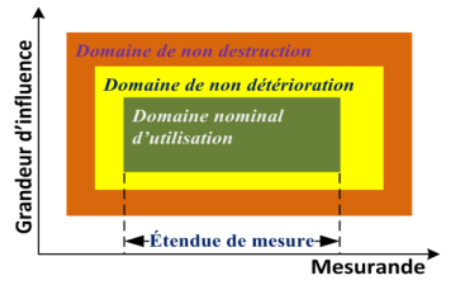
\includegraphics[width=0.4\linewidth]{./images/006-etendue-de-mesure.png}
            \caption{Étendue de mesure}
        \end{figure}
        
        \subsection{Temps de réponse}
        \paragraph{}
        La rapidité d'un capteur est le temps de réaction entre la variation de la grandeur physique qu'il mesure et l'instant où l'information est prise en compte par la partie commande.

        \begin{figure}[H]
            \centering
            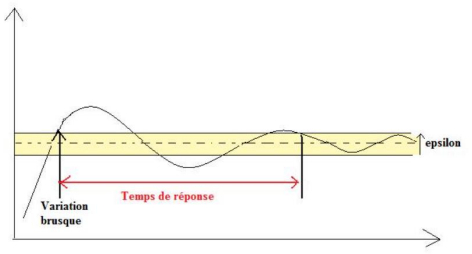
\includegraphics[width=0.5\linewidth]{./images/007-rapidite.png}
            \caption{Rapidité}
        \end{figure}

        \subsection{Grandeurs d'influence}
        \paragraph{}
        Les grandeurs d'influence sont des grandeurs physiques autres que le mesurande dont la variation peut modifier la réponse du capteur (température, pression, humidité, etc). Il est nécessaire de les réduire, de les stabiliser et/ou de les compenser.


    \section{Étalonnage des capteurs}
    \paragraph{}
    L'étalonnage d'un capteur consiste à établir la relation qui existe entre la grandeur à mesurer et la grandeur élactrique de sortie. Si cette relation est graphique, elle est représentée par une courbe d'étalonnage et si cette relation est algébrique, elle l'est par l'équation caractéristique du capteur.

    \begin{figure}[H]
        \centering
        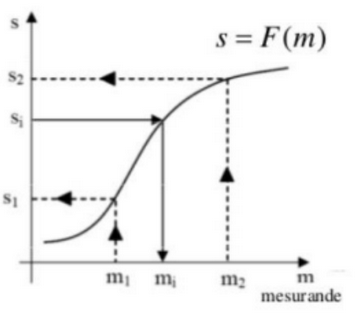
\includegraphics[width=0.3\linewidth]{./images/008-etalonnage.png}
        \caption{Étalonnage}
    \end{figure}

        \subsection{Étalonnage à l'aide d'Excel}
        \paragraph{}
        A partir des points de mesure, le logiciel Excel va nous permettre de tracer la courbe de tendance et de donner son équation. A partir de celle-ci, on pourra par la suite connaître une température quelconque de la CTN par la mesure de sa résistance.

        \paragraph{}
        Pour étalonner correctement un capteur, il est parfois nécessaire de comparer les valeurs lues aux valeurs correctes attendues afin de corriger les erreurs : c'est le calibrage de l'appareil.

        \paragraph{L'étalonnage simple} consiste à fixer tous les paramètres d'influence et ne faire varier que la seule grandeur à mesurer.

        \paragraph{L'étalonnage multiple} tient compte de toutes les grandeurs d'influence, il s'agit d'un ensemble d'étalonnages successifs qui détermine la dépendance de la grandeur principale vis-à-vis des grandeurs d'influence.

        \paragraph{L'étalonnage absolu} consiste à fournir les valeurs de la grandeur à mesurer par des étalons ou par des éléments de référence de très grande précision.

        \paragraph{L'étalonnage relatif} est l'utilisation d'un capteur dont on connaît la courbe d'étalonnage et dont la stabilité est assez grande. Le capteur à étalonner et le capteur étalonné sont soumis tous les deux aux mêmes contraintes et dans les mêmes conditions. C'est alors par comparaison qu'on établit la courbe d'étalonnage du capteur.

\newpage
\section{Capteurs passifs}
\paragraph{}
Impédance ou résistance dont la valeur varie avec la grandeur physique. Nécessite une alimentation.

\paragraph{}
L'impédance varie par :
\begin{itemize}
    \item la variation des dimensions du capteur
    \item la modification de propriétés électriques des matériaux
\end{itemize}

\subsection{La résistivité}
\paragraph{}
La résistivité d'un matériau, notée $\rho$, est égale à la résistance d'un tronçon de matériau d'un mètre de longueur et d'un mètre carré de section. Elle s'exprime en [\si{\ohm\meter}] :
$$R = \rho\frac{L}{S}$$

\paragraph{}
La résistivité représente la capacité du matériau à s'opposer à la circulation du courant électrique.

\paragraph{}
Exemples de résistivités d'isolants :
\begin{table}[H]
    \centering
    \begin{tabular}{l l}
        Eau pure & $1,8.10^5 \si{\ohm\meter}$\\
        \hline
        Verre & $10^{17} \si{\ohm\meter}$\\
        \hline
        Air & variable\\
        \hline
        Polystyrène & $10^{20} \si{\ohm\meter}$\\
    \end{tabular}
\end{table}

\paragraph{}
Exemples de résistivités de métaux :
\begin{table}[H]
    \centering
    \begin{tabular}{l l}
        Argent & $16.10^{-9} \si{\ohm\meter}$\\
        \hline
        Cuivre & $17.10^{-9} \si{\ohm\meter}$\\
        \hline
        Fer & $100.10^{-9} \si{\ohm\meter}$\\
        \hline
        Plomb & $208.10^{-9} \si{\ohm\meter}$\\
    \end{tabular}
\end{table}

\paragraph{}
La résistivité évolue avec la température :
\begin{itemize}
    \item Dans le cas des métaux (PT100), elle croit linéairement avec la température : $\rho = \rho_0\left(1 + \alpha_0\left(\theta - \theta_0\right)\right)$
    \item Dans le cas des semi-conducteurs, elle décroît avec la température. Elle peut aussi dépendre de la quantité de rayonnement absorbé par le composant.
\end{itemize}

\paragraph{}Exemples de coefficients de température de métaux pour $\theta_0 = \SI{20}{\celsius}$ :
\begin{table}[H]
    \centering
    \begin{tabular}{l l}
        \textbf{Métal} & \textbf{$\alpha [10^{-3}\si{\per\kelvin}]$}\\
        \hline
        Argent & 3,85\\
        Cuivre & 3,93\\
        Aluminium & 4,03\\
        Plomb & 4,2\\
        Tungstène & 4,5\\
        Nickel & 5,37\\
        Fer & 6,5\\
    \end{tabular}
\end{table}

\subsection{La permittivité (diélectrique)}
\paragraph{}
La permittivité (diélectrique) ou constante diélectrique, notée $\epsilon$, est une propriété électrique d'un milieu. Elle caractérise la réponse d'un milieu donné à un champ électrique appliqué :
$$\epsilon = \epsilon_r \epsilon_0$$
$$\epsilon_0 = 8,85.10^{-12} \si{\farad\per\meter}$$

\paragraph{}
Permittivités relatives typiques isolants :
\begin{table}[H]
    \centering
    \begin{tabular}{l l}
        \textbf{Matériau} & \textbf{Permittivité relative $\epsilon_r$}\\
        \hline
        vide & 1\\
        air sec & 1,0006\\
        papier & 2,3\\
        verre standard & 5\\
        eau & 78,5\\
    \end{tabular}
\end{table}

\subsection{La perméabilité magnétique}
\paragraph{}
La perméabilité caractérise la faculté d'un matériau à modifier un champ magnétique :
$$\mu = \mu_0 \mu_r$$

\begin{itemize}
    \item $\mu$ = la perméabilité magnétique du matériau [\si{\henry\per\meter}]
    \item $\mu_0$ = la perméabilité du vide = $4\pi.10^{-7}$ [\si{\henry\per\meter}]
    \item $\mu_r$ = la perméabilité relative
\end{itemize}

\begin{figure}[H]
    \centering
    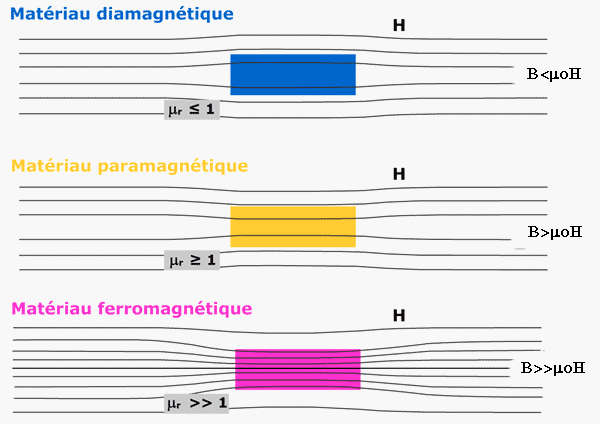
\includegraphics[width=0.7\linewidth]{./images/permeabilite_magnetique_m.png}
    \caption{Perméabilité magnétique}
\end{figure}

\subsubsection{Magnétisme}
\paragraph{Les matériaux diamagnétiques} s'aimantent faiblement dans le sens opposé au champ magnétisant (cet effet cesse dès que le champ magnétique est supprimé).

\paragraph{Les matériaux paramagnétiques} s'aimantent faiblement dans le même sens que le champ magnétisant (cet effet cesse dès que le champ magnétique est supprimé).

\paragraph{Les matériaux ferromagnétiques} peuvent être facilement magnétisés.

\subsubsection{Champ magnétique}
\paragraph{}
Si le régime du matériau est dit linéaire, la champ magnétique $$B = \mu . H$$
\begin{itemize}
    \item B = champ (d'induction) magnétique [\si{\tesla}] (1 Gauss [G] = $10^{-4}$ \si{\tesla})
    \item H = champ d'excitation magnétique
\end{itemize}

\paragraph{}Exemples :
\begin{itemize}
    \item Bterrestre : 0,5G
    \item Petit aimant : 2kG à 4kG
    \item Petit aimant néodyme : 13kG
\end{itemize}

\paragraph{}
Perméabilité magnétique relative de matériaux ferromagnétiques à \SI{20}{\celsius} :
\begin{table}[H]
    \centering
    \begin{tabular}{c c}
        \textbf{Matériaux} & \textbf{$\mu_r$}\\
        \textbf{ferromagnétiques} & \textbf{(valeur max)}\\
        \hline
        Cobalt & 250\\
        Fer & 5000\\
        Mu-métal & 100 000\\
        Nickel & 600\\
    \end{tabular}
\end{table}

\subsection{Effets physiques mesurés par les capteurs passifs}
\begin{table}[H]
    \centering
    \begin{tabular}{c c c}
        \textbf{Mesurande} & \textbf{Caractéristiques électriques sensibles} & \textbf{Types de matériaux utilisés}\\
        \hline
        Température & Résistivité & Métaux : platine, nickel, cuivre\\
        Très basse température & Constante diélectrique & Verres\\
        \hline
        Flux lumineux & Résistivité & Semi-conducteur\\
        \hline
        Déformation & Résistivité & Alliages de nickel, silicium dopé\\
        & Perméabilité magnétique & Alliages ferromagnétiques\\
        \hline
        Position & Résistivité & Matériaux magnéto-résistants :\\
         &  & bismuth, antimoine d'indium\\
        \hline
        Humidité & Résistivité & Chlorure de lithium\\
         & Constante diélectrique & Alumine, polymères\\
        \hline
        Niveau & Constante diélectrique & Liquides isolants\\
    \end{tabular}
\end{table}


\subsection{Capteurs à résistance variable}
\paragraph{}
La résistance d'un conducteur :
$$R = \rho \frac{l}{S} = \rho_0 (1 + \alpha \theta) \frac{l}{S}$$

\paragraph{}
Si $\alpha$ est constant, alors R = f(l, $\Theta$).

\subsubsection{Capteurs potentiométriques}
\paragraph{}
Le déplacement est donné par la position du curseur.

\begin{figure}[H]
    \centering
    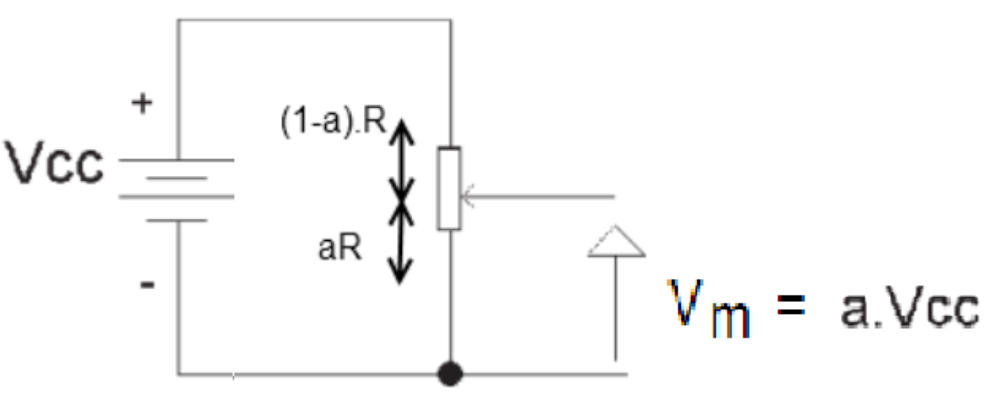
\includegraphics[width=0.5\linewidth]{./images/potentiometre.png}
\end{figure}

\paragraph{}
Inconvénients : usure mécanique (durée de vie $\pm$ 50 000 man\oe uvres). On les remplace par des capteurs magnéto-résistifs plus résistants et plus précis.

\subsubsection{Capteurs à jauge de déformation}
\paragraph{}
Ce capteur est collé sur la pièce et permet de traduire la déformation de celle-ci en variation de résistance électrique :
$$\frac{\Delta R}{R} = K \frac{\Delta L}{L}$$
\begin{itemize}
    \item K = facteur de jauge
\end{itemize}

\begin{figure}[H]
    \centering
    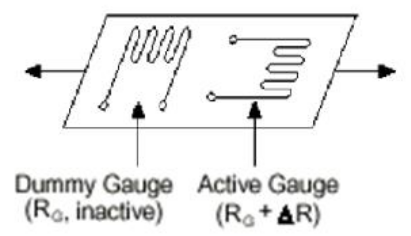
\includegraphics[width=0.3\linewidth]{./images/jauge-contrainte.png}
\end{figure}

\paragraph{}
La jauge de contrainte peut être utilisée avec des fréquences élevées ( $<$ 50 \si{\kilo\hertz}). Son élongation maximale est de 3 à 5\%.

\paragraph{}
Ces capteurs permettent de mesurer des forces, des pressions, etc.

\subsubsection{Capteurs magnéto-résistifs}
\paragraph{}
La résistance électrique (la résistivité) du matériau varie en fonction de la direction du champ magnétique appliqué.

\begin{figure}[H]
    \centering
    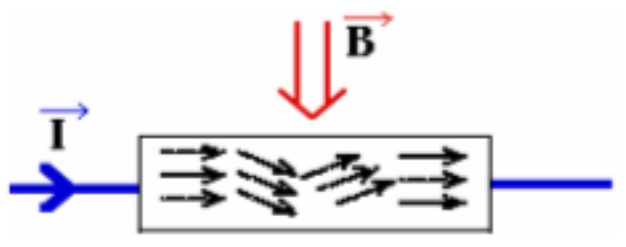
\includegraphics[width=0.3\linewidth]{./images/magnetoresistif.png}
\end{figure}

\paragraph{}
Ces capteurs permettent de détecter le mouvement de matières ferromagnétiques : mesure de vitesse, détection de roues dentées, contrôle de rotation.

\paragraph{}
Exemples : 2SSM13, SM351LT, SM353LT.

\subsubsection{Capteurs de température résistifs}
\paragraph{Les thermo-résistances} fonctionne par variation de la résistivité de certains matériaux (argent, cuivre, nickel, or, platine, etc.) selon la température. La résistance augmente de manière sensiblement linéaire avec la température.

\paragraph{}
Exemple : PT 100

\subsection{Capteurs capacitifs}
\paragraph{}Principe :
\begin{figure}[H]
    \centering
    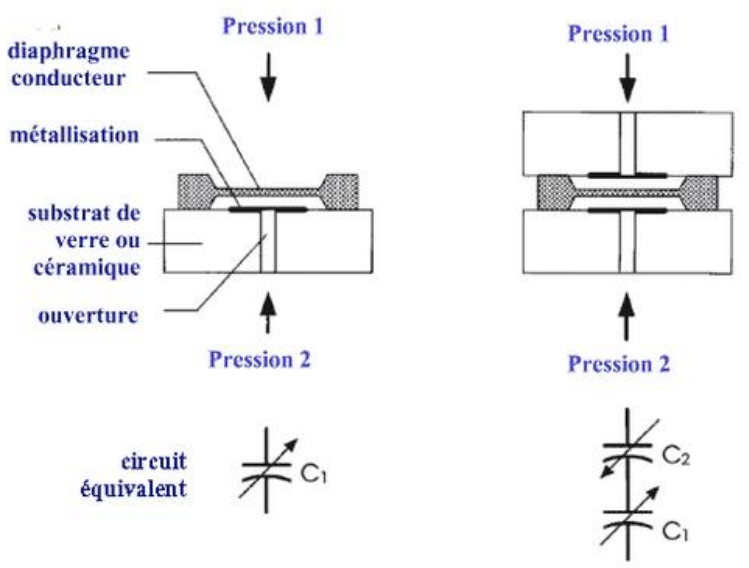
\includegraphics[width=0.6\linewidth]{./images/capteur-capacitif.png}
\end{figure}

\paragraph{}
Exemple : capteur de niveau Serie 90 - KAS-90-...-P-... de Rechner Sensors.

\newpage
\section{Capteurs actifs}
\paragraph{}
Les capteurs actifs génèrent directement une tension, un courant ou une charge à partir de la grandeur physique. Ils utilisent un principe physique qui convertit directement l'énergie fournie par le mesurande en énergie électrique.

\subsection{Effets physiques mesurés par les capteurs actifs}
\begin{table}[H]
    \centering
    \begin{tabular}{c c c c}
        & \textbf{Énergie propre} & & \textbf{Grandeur}\\
        \textbf{Mesurande} & \textbf{du mesurande} & \textbf{Principe physique} & \textbf{de sortie}\\
        \hline
        Température & Énergie thermique & Effet thermoélectrique & Tension\\
         &  & Effet pyroélectrique & Charge\\
        \hline
        Flux lumineux & Énergie électromagnétique & Effet photo-émissif & Courant\\
        &  & Effet photovoltaïque & Tension\\
        &  & Effet photoélectrique & Tension\\
        \hline
        Force & & & \\
        Pression & & Effet piézoélectrique & Charge \\
        Accélération & Énergie mécanique & & \\
        Vitesse & & Effet d'induction électromagnétique & Tension \\
        Position & & Effet Hall & Tension \\
    \end{tabular}
\end{table}

\subsection{Thermocouples}
\paragraph{}
Un thermocouple est créé dès lors que deux métaux différents entrent en contact, ce qui produit une faible tension en circuit ouvert au point de contact, qui varie en fonction de la température. Cette tension thermo-électrique est connue sous le nom de tension de Seebeck.
$$E = S (\theta_1 - \theta_2)$$
\begin{itemize}
    \item E = fém obtenue
    \item $\theta_1$ = température soudure chaude
    \item $\theta_2$ = température soudure froide
    \item S = coefficient de Seebeck
\end{itemize}

\paragraph{}
Les câbles d'extension sont des conducteurs de même nature que les fils du thermocouple. Les câbles de compensation sont des conducteurs de nature différente que les fils du thermocouple.

\subsubsection{Choix pour la mesure de la température}
\begin{table}[H]
    \centering
    \begin{tabular}{l | l | l | l}
        \textbf{Critères} & \textbf{Thermocouple} & \textbf{RTD} & \textbf{Thermistance}\\
        \hline
        Échelle des temp. & $\SI{-267}{\celsius}$ à $\SI{2316}{\celsius}$ & $\SI{-240}{\celsius}$ à $\SI{649}{\celsius}$ & $\SI{-100}{\celsius}$ à $\SI{500}{\celsius}$\\
        \hline
        Précision & Bonne & Optimale & Bonne\\
        \hline
        Linéarité & Meilleure & Optimale & Bonne\\
        \hline
        Sensibilité & Bonne & Meilleure & Optimale \\
        \hline
        Coût & Optimal & Bon & Meilleur\\
    \end{tabular}
\end{table}

\paragraph{}
Les thermocouples sont robustes et à des prix abordables. Ils ont un temps de réponse rapide mais sont moins précis et les moins stables et sensibles des capteurs. En outre, ils lisent uniquement les différences relatives de températures entre l'extrémité et les conducteurs alors que les RTD et les thermistances lisent la température absolue.

\paragraph{}
Les RTD sont le choix privilégié pour la répétabilité. Ils sont aussi plus stables et précis. Cependant, leur temps de réponse est lent et comme ils requièrent une source de courant ils ont une quantité faible d'auto-échauffement.

\paragraph{}
Les thermistances ont un temps de réponse rapide et sont relativement peu onéreuses, mais elles sont fragiles et ont une gamme de mesure limitée. Elles requièrent aussi une source de courant et ont un taux d'auto-échauffement plus important que les RTD. En outre, elles sont non-linéaires.



\newpage
\section{Capteurs intégrés}
\paragraph{}
On intègre sur le même substrat de silicium le capteur et le conditionnement du signal. Cela permet de réduire l'encombrement de la chaîne de mesure, de faciliter la mise en \oe uvre du capteur et de favoriser la normalisation des capteurs.

\paragraph{}
Exemple : LM35

\newpage
\section{Capteurs intelligents}
\paragraph{}
On intègre sur la même puce le capteur et les circuits associés pour le traitement et la transmission de l'information. Cela permet de commander à distance le capteur, de gérer plusieurs capteurs, de gérer différentes mesures et de les corriger.

\newpage
\section{Conditionnement du signal}
\subsection{Raccordement}
\subsubsection{Raccordement direct (2 fils)}
\paragraph{}
Mesurer une résistance faible requiert de s'affranchir des résistances de contact et des conducteurs.

\begin{figure}[H]
    \centering
    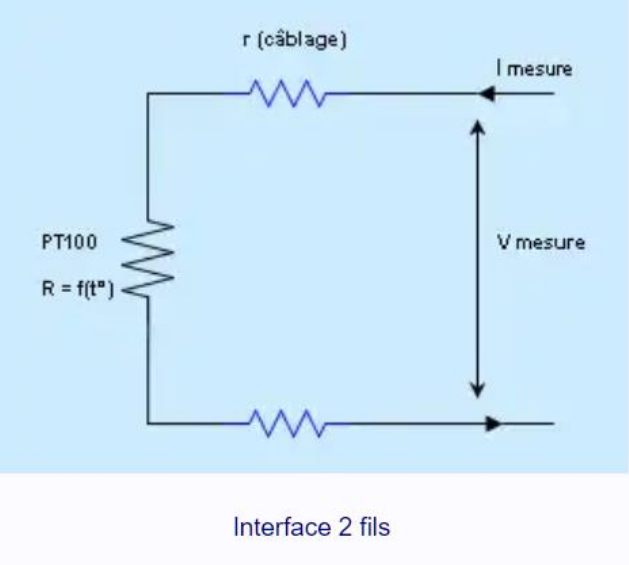
\includegraphics[width=0.43\linewidth]{./images/2fils.png}
\end{figure}

\paragraph{}
Une résistance se mesure par le rapport $\frac{U}{I}$.

\subsubsection{Interface à 3 fils}
\paragraph{}
Le principe du 3 fils consiste à mesurer la chute de tension dans un des deux fils, la doubler (ce qui implique des fils identiques) et la soustraire.

\begin{figure}[H]
    \centering
    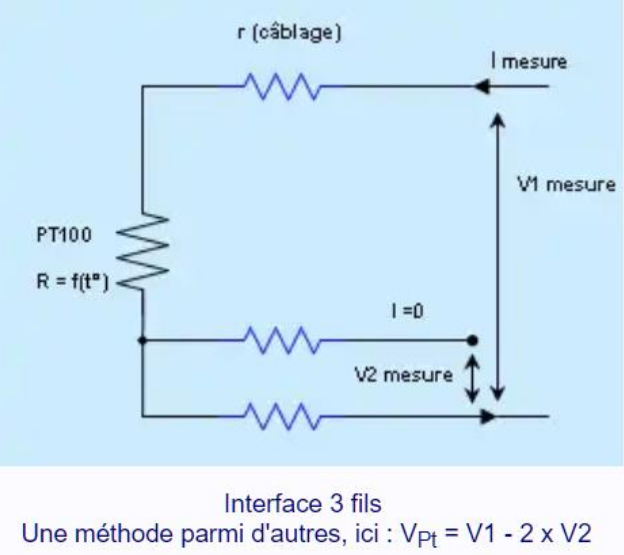
\includegraphics[width=0.43\linewidth]{./images/3fils.png}
\end{figure}

\subsubsection{Interface à 4 fils}
\paragraph{}
Deux sont utilisés pour alimenter la sonde, les deux autres sont raccordés à la mesure. Les résistances des fils n'interviennent plus.

\begin{figure}[H]
    \centering
    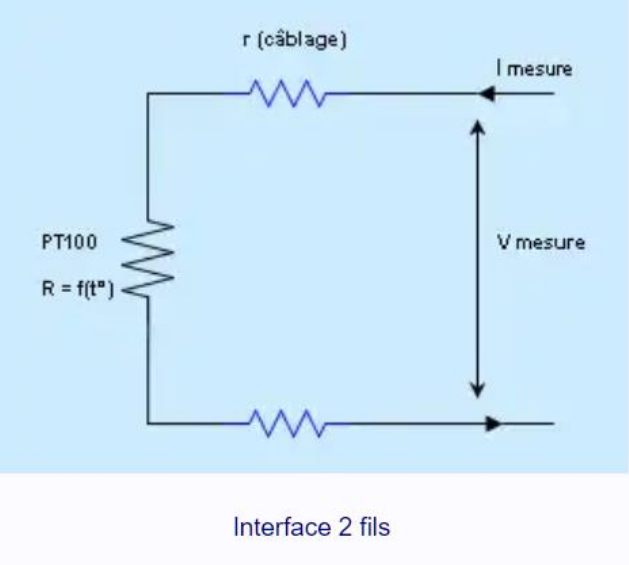
\includegraphics[width=0.43\linewidth]{./images/2fils.png}
\end{figure}

\paragraph{Remarque :} pas raccordable sur automate, réservé à l'étalonnage.

\subsection{Pont de Wheatstone}
\paragraph{}
Le pont de Wheatstone est utilisé pour mesurer les petites variations de résistance électrique (e.g. pour une jauge de contrainte). Si la tension de sortie est nulle, on a :
$$\frac{R_1}{R_4} = \frac{R_2}{R_3} = r$$

\begin{figure}[H]
    \centering
    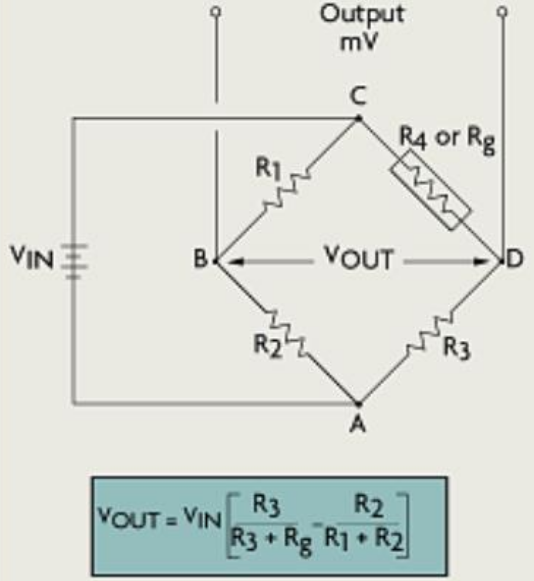
\includegraphics[width=0.35\linewidth]{./images/wheatstone.png}
\end{figure}

\begin{figure}[H]
    \centering
    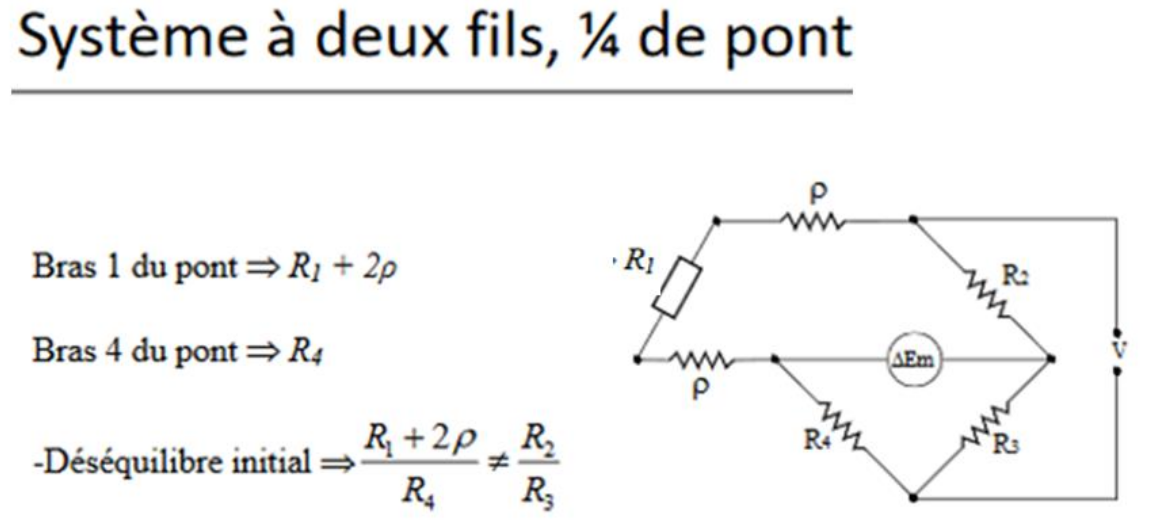
\includegraphics[width=0.65\linewidth]{./images/wheatstone-2fils.png}
\end{figure}

$$\frac{R_1}{R_4} = \frac{R_2}{R_3} = r$$

\begin{figure}[H]
    \centering
    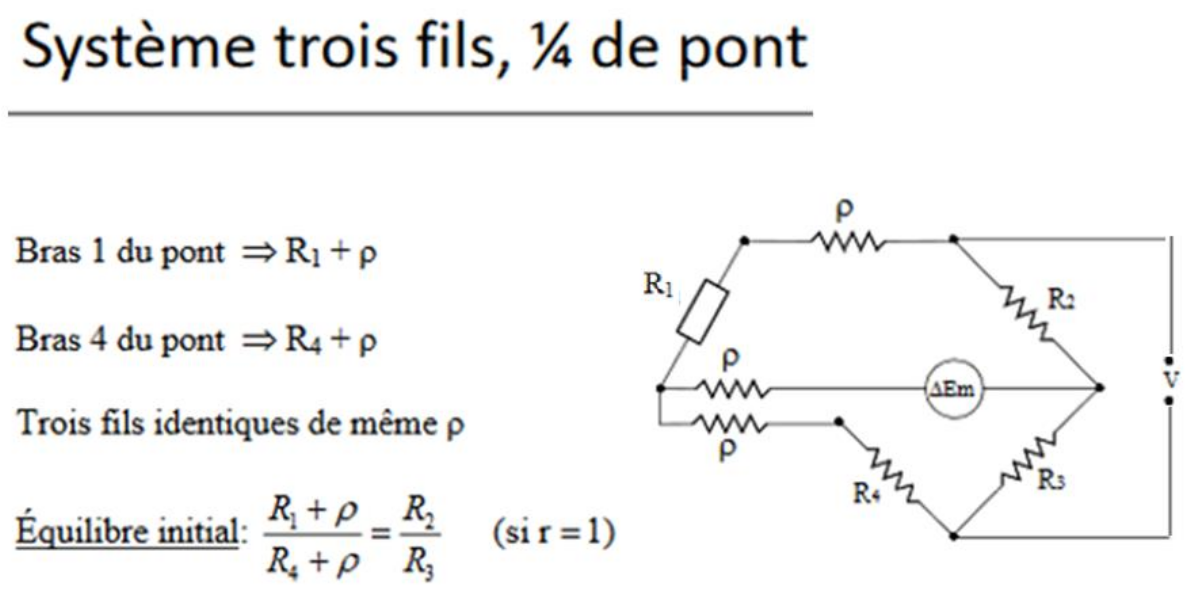
\includegraphics[width=0.65\linewidth]{./images/wheatstone-3fils-1.png}
\end{figure}

\begin{figure}[H]
    \centering
    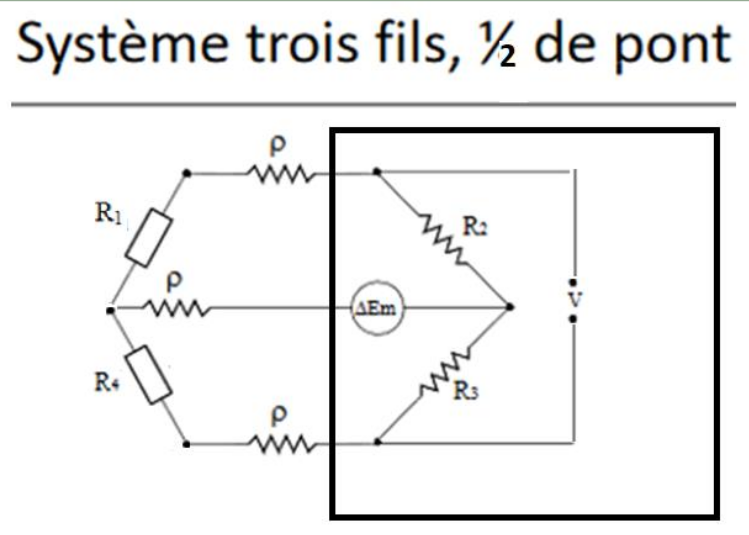
\includegraphics[width=0.45\linewidth]{./images/wheatstone-3fils-3.png}
\end{figure}

\paragraph{}
Deux jauges actives : R1 et R4. Le demi-pont est relié à l'amplificateur par trois fils : deux pour l'alimentation, et le troisième pour la mesure.

\paragraph{}
Dans ce montage, le câblage n'a pas d'influence sur l'équilibre du pont. L'effet thermique est également compensé, mais pas les pertes en ligne.



\newpage
\section{Chaîne de mesure}
\paragraph{}
Une chaîne de mesure est la suite des éléments d'un système de mesure qui constitue un seul chemin du signal depuis le capteur jusqu'à l'élément de mesure.

\paragraph{}
Elle comprend :
\begin{itemize}
    \item un capteur,
    \item un signal qui suit un chemin dans la succession des éléments,
    \item un élément de sortie qui rend une indication sous forme analogique ou numérique.
\end{itemize}

\paragraph{}
Un appareil de mesure est un chaîne de mesure.

\subsection{Chaîne de mesure analogique}
\paragraph{}
Un signal analogique est basé sur une grandeur physique qui varie de façon continue et dont la valeur varie de façon analogue à la grandeur d'entrée.

\begin{figure}[H]
    \centering
    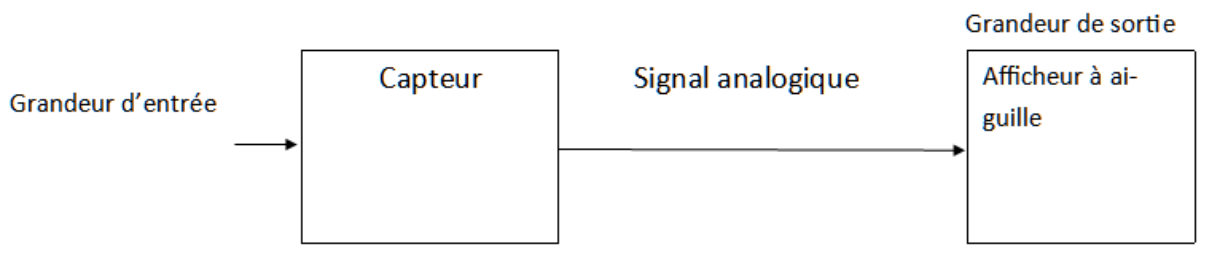
\includegraphics[width=0.8\linewidth]{images/chaine-mesure-analogique.png}    
\end{figure}

\paragraph{}
La graduation du cadran est effectuée lors de l'étalonnage de la chaîne de mesure.

\subsection{Chaîne de mesure numérique}
\paragraph{}
Un signal numérique est un signal restitué sous la forme d'un nombre à partir d'un signal analogique.

\begin{figure}[H]
    \centering
    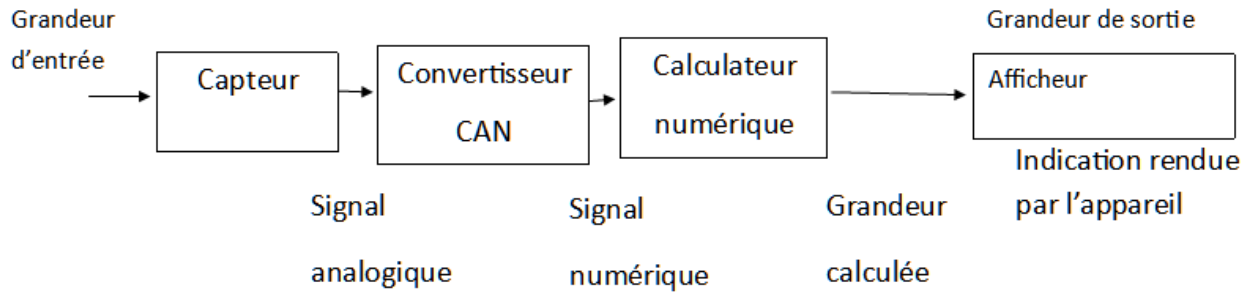
\includegraphics[width=0.9\linewidth]{images/chaine-mesure-numerique.png}    
\end{figure}

Elle se décompose comme suit :
\begin{itemize}
    \item Capteur
    \item Convertisseur CAN
    \item Calculateur numérique
    \item Afficheur numérique
\end{itemize}

\subsubsection{Capteur}

\begin{figure}[H]
    \centering
    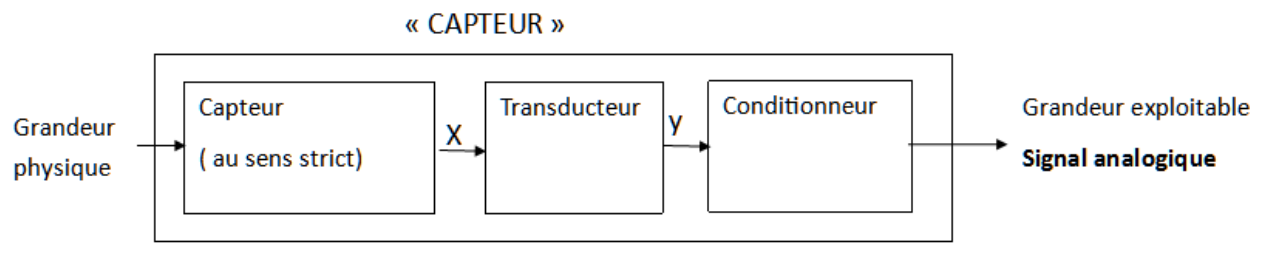
\includegraphics[width=0.9\linewidth]{images/capteur.png}    
\end{figure}

\begin{itemize}
    \item \textbf{L'élément capteur} : soumis à l'action de la grandeur d'entrée
    \item \textbf{Transducteur} : élément faisant correspondre à la grandeur d'entrée une autre grandeur de sortie
    \item \textbf{Conditionneur} : élément qui fournit une grandeur exploitable
\end{itemize}

\paragraph{}
Exemple :
\begin{figure}[H]
    \centering
    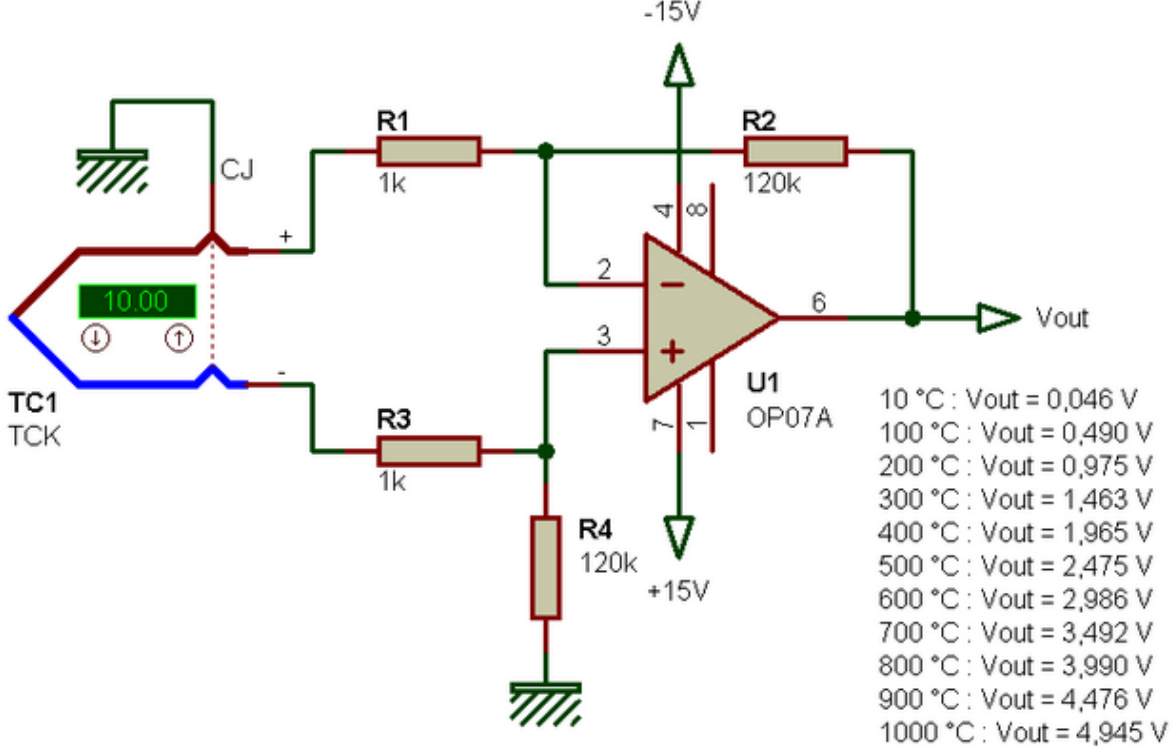
\includegraphics[width=0.9\linewidth]{images/ex-conditionneur.png}    
\end{figure}

\paragraph{}
Mais aussi : conditionneur de balance, ex 2 conditionneur, pont de Wheatstone, etc.

\subsubsection{Convertisseur CAN}
\paragraph{}
A partie d'un signal analogique (tension ou courant), le convertisseur restitue un signal numérique utilisable par un calculateur.

\begin{figure}[H]
    \centering
    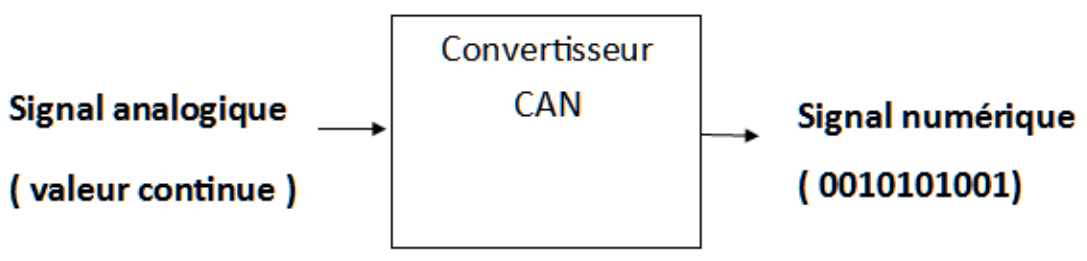
\includegraphics[width=0.6\linewidth]{images/CAN.png}    
\end{figure}

\paragraph{Signal numérique}
\paragraph{}
\textbf{La numérisation d'un signal} ou le passage de l'analogique au numérique repose sur trois étapes successives : l'\textbf{échantillonnage}, la \textbf{quantification} et le \textbf{codage}.

\paragraph{}
Un signal numérique est une suite discrète de valeurs numériques (en général des entiers).

\paragraph{Échantillonnage}
\paragraph{}
L'échantillonnage consiste à relever à intervalle régulier la valeur d'une grandeur physique. La fréquence d'échantillonnage est le nombre d'échantillons par unité de temps. Le signal analogique de départ est continu en temps et en amplitude.

\begin{figure}[H]
    \centering
    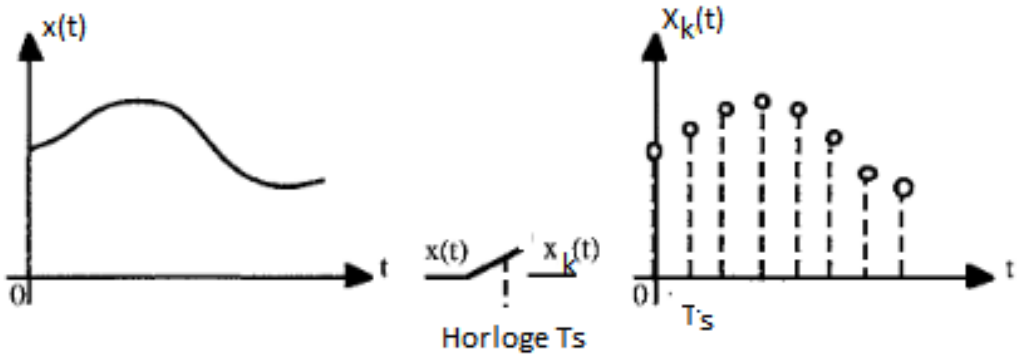
\includegraphics[width=0.6\linewidth]{images/echantillonnage.png}    
\end{figure}

\paragraph{}
En pratique, on utilise le théorème de Shannon pour déterminer la fréquence d'échantillonnage :
$$f_S \ge 2f_M$$ ou $$T_S \le \frac{1}{2f_M}$$
\begin{itemize}
    \item $f_M$ = fréquence maximale d'un signal continu
    \item $\frac{1}{2f_M}$ = période d'échantillonnage critique
\end{itemize}

\paragraph{}
Transformation d'un signal continu en un signal discret :
\begin{figure}[H]
    \centering
    \begin{subfigure}{\textwidth}
        \centering
        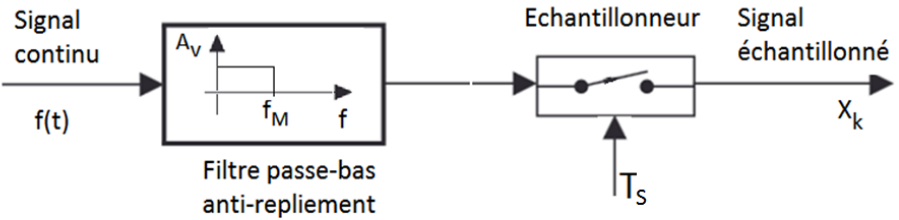
\includegraphics[width=0.8\linewidth]{./images/CAN1.png}
    \end{subfigure}
    \begin{subfigure}{.4\textwidth}
        \centering
        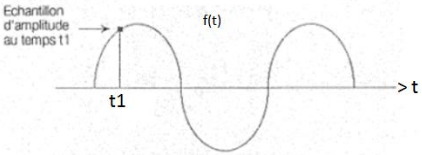
\includegraphics[width=\linewidth]{./images/CAN2.png}
    \end{subfigure}
    \begin{subfigure}{.4\textwidth}
        \centering
        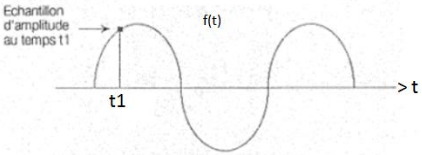
\includegraphics[width=\linewidth]{./images/CAN2.png}
    \end{subfigure}
\end{figure}

\paragraph{Quantification}
\paragraph{}
Un signal analogique dont l'amplitude ne peut prendre que des valeurs entières précises est dit quantifié.

\begin{figure}[H]
    \centering
    \begin{subfigure}{.3\textwidth}
        \centering
        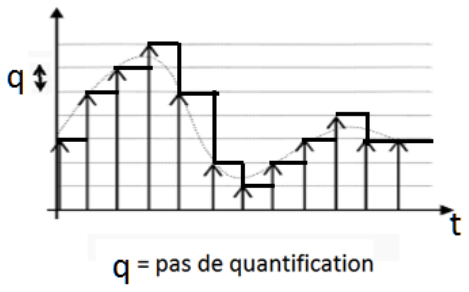
\includegraphics[width=\linewidth]{./images/quantification1.png}
    \end{subfigure}
    \begin{subfigure}{.6\textwidth}
        \centering
        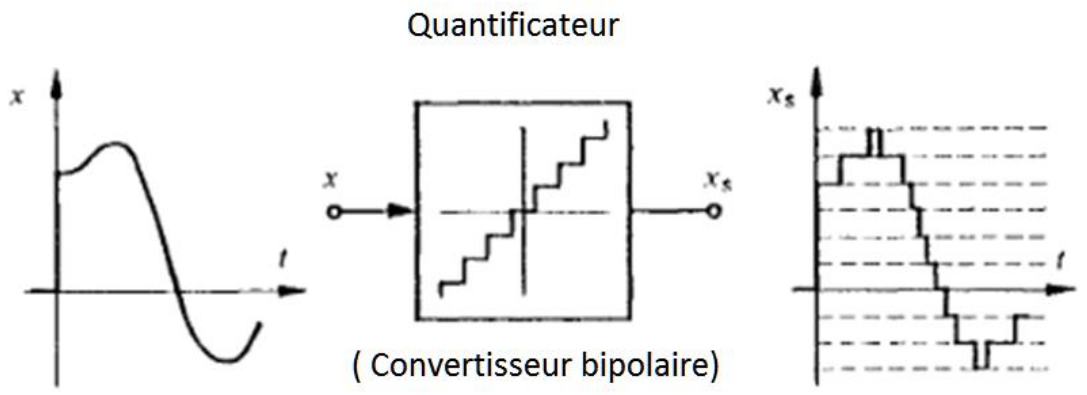
\includegraphics[width=\linewidth]{./images/quantification2.png}
    \end{subfigure}
\end{figure}
\begin{figure}[H]
    \centering
    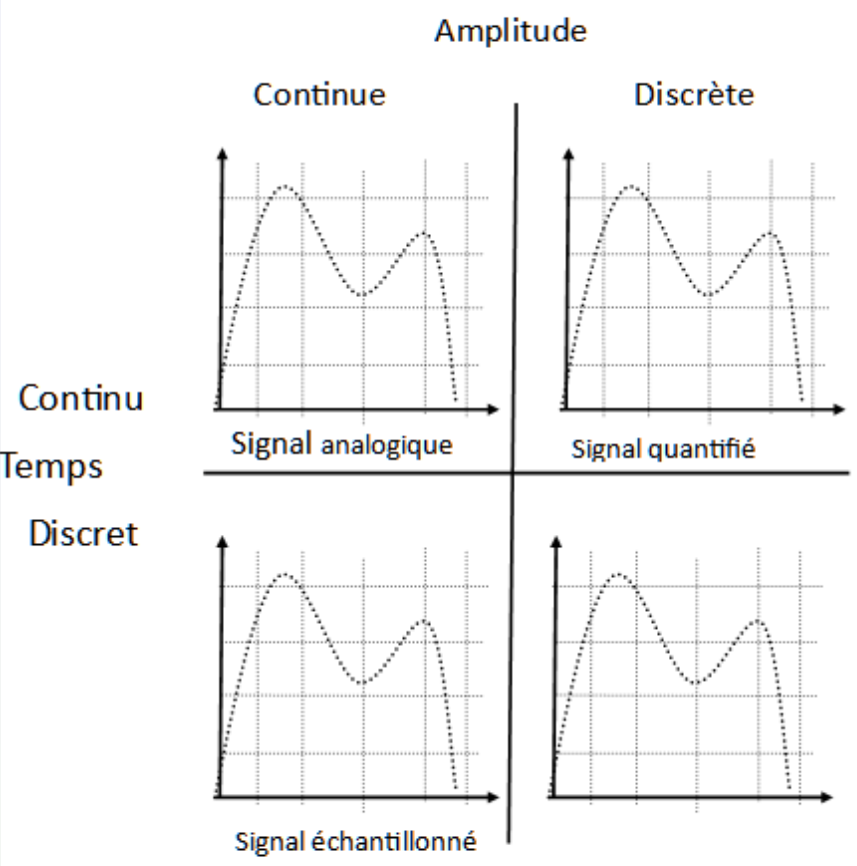
\includegraphics[width=0.6\linewidth]{images/quantification3.png}
\end{figure}

\paragraph{Codage}\
\begin{figure}[H]
    \centering
    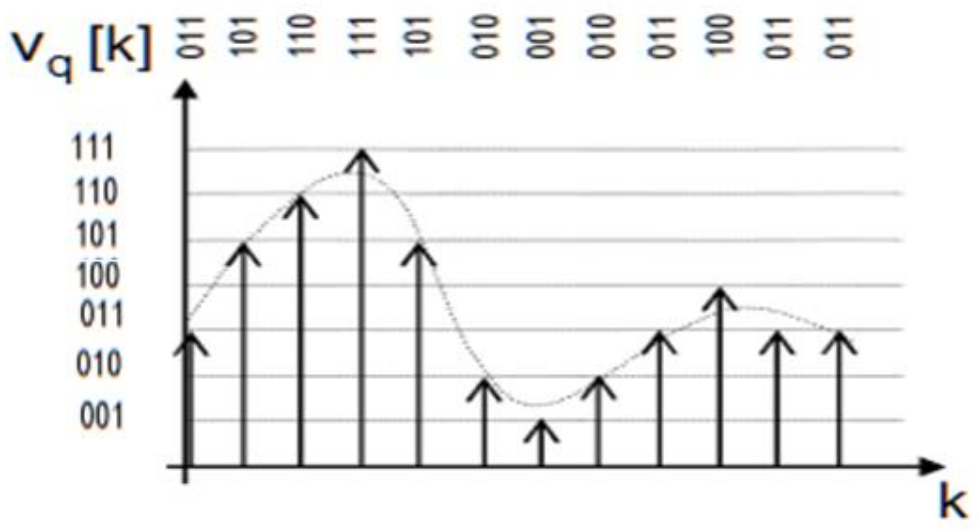
\includegraphics[width=.5\linewidth]{images/codage.png}
\end{figure}

\paragraph{Convertisseur CAN (ou ADC)}
\paragraph{}
Un convertisseur analogique/numérique (CAN) est un dispositif électronique permettant la conversion d'un signal analogique en un signal numérique.

\newpage
\paragraph{}
Exemple : CAN unipolaire 3 bits = 8 niveaux
\begin{figure}[H]
    \centering
    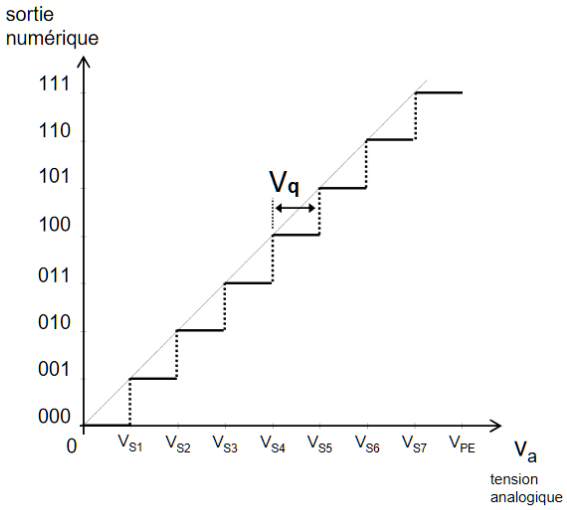
\includegraphics[width=.5\linewidth]{images/CAN-3bits.png}
\end{figure}

\paragraph{}
Exemple : Convertisseur flash
\begin{figure}[H]
    \centering
    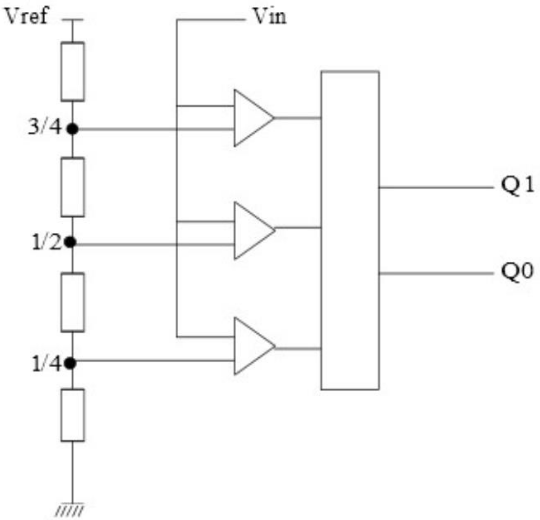
\includegraphics[width=.5\linewidth]{images/convertisseur-flash.png}
\end{figure}

\newpage
\paragraph{}
Comparaison de convertisseurs CAN :
\begin{figure}[H]
    \centering
    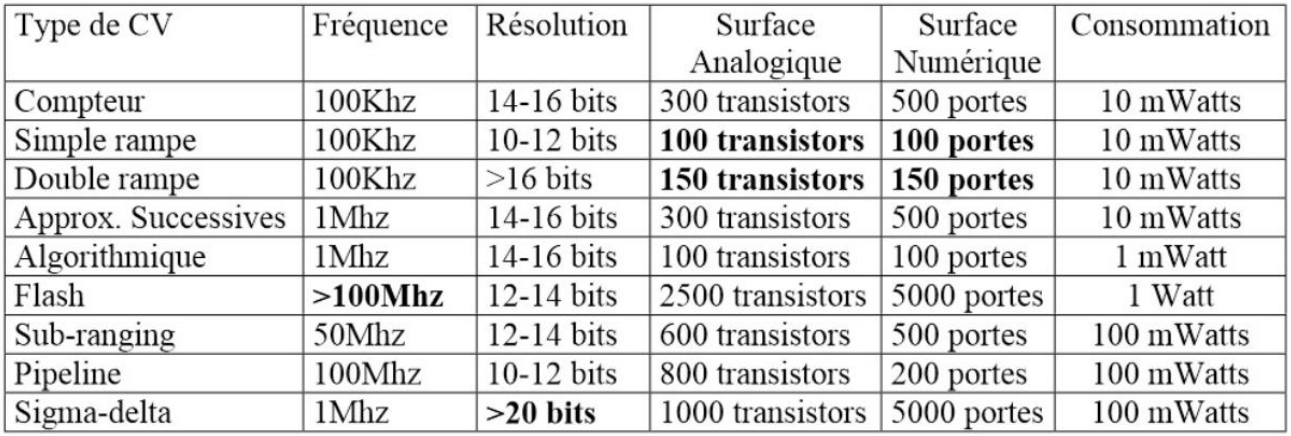
\includegraphics[width=\linewidth]{images/CAN-comp.png}
\end{figure}

\paragraph{}
Exemple : AD7896 Convertisseur analogique-numérique 12bits à sortie série

\begin{figure}[H]
    \centering
    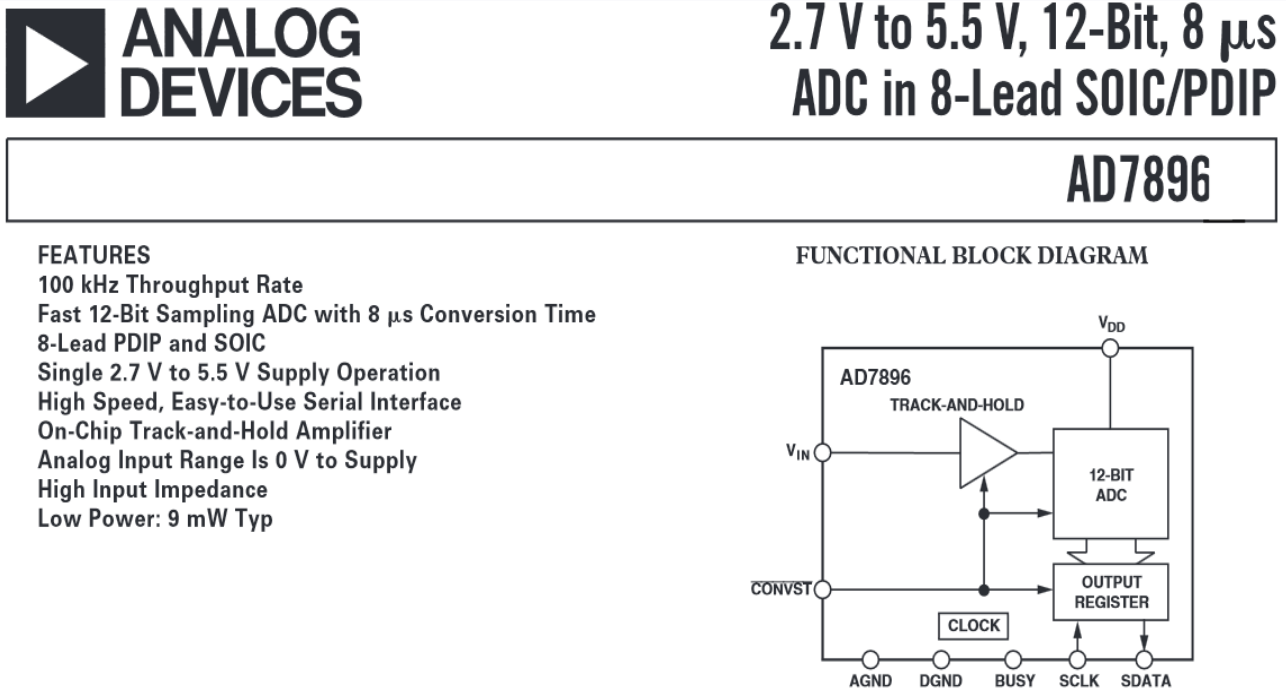
\includegraphics[width=0.9\linewidth]{images/AD7896.png}
\end{figure}

\subsubsection{Calculateur numérique}
\paragraph{}
Le calculateur numérique permet de transformer le signal numérique provenant du CAN en une indication correspondant à la grandeur d'entrée (masse, force, température, etc).

\paragraph{}
Pour réaliser cette fonction, il doit être étalonné. L'étalonnage est initialement réalisé par le constructeur à l'aide d'étalons. Il établit la relation entre les valeurs numériques du CAN et les valeurs des étalons.

\paragraph{}
Lors d'une mesure, le calculateur utilise une relation d'étalonnage pour rendre une indication : c'est le mesurage.






\subsubsection{Afficheur numérique}


\subsubsection{Erreurs d'une chaîne de mesure}
\paragraph{}
La valeur d'un mesurage ne peut être évaluée que par la chaîne de mesurage. 

\paragraph{L'erreur de mesure} est l'écart entre la valeur mesurée et la valeur de référence. Elle est donnée par la somme de l'erreur systématique et de l'erreur aléatoire.

\paragraph{L'erreur systématique} se détermine comme un décalage constant entre la valeur du mesurande et la valeur de référence.

\paragraph{L'erreur aléatoire} ou erreur accidentelle sont les écarts non constants entre al valeur de référence et la valeur mesurée pour une même valeur de mesurande.




\end{document}